\documentclass[tikz,border=8pt]{standalone}
\usepackage[T1]{fontenc}\usepackage{lmodern}\usepackage{pgfplots}\pgfplotsset{compat=1.18}
\begin{document}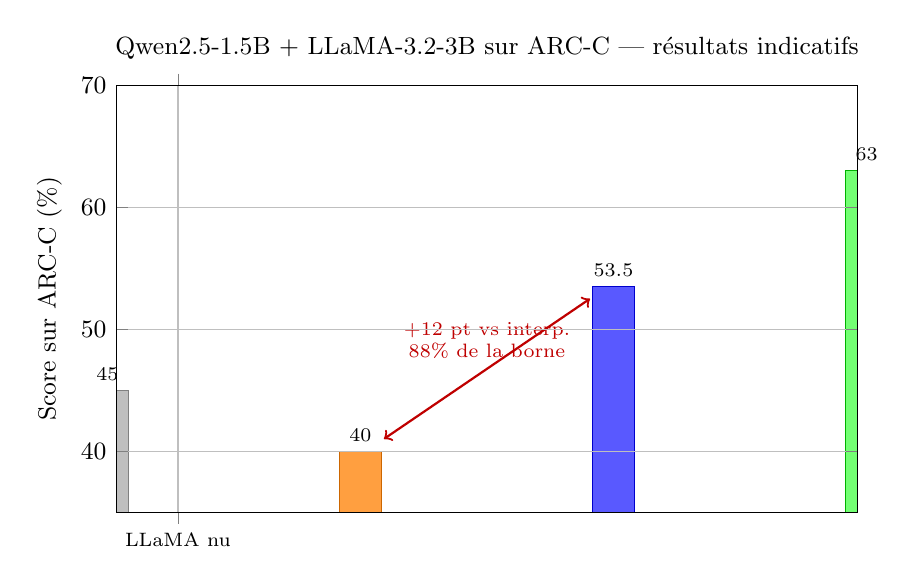
\begin{tikzpicture}
\begin{axis}[ybar,width=11cm,height=7cm,font=\small,title={Qwen2.5-1.5B + LLaMA-3.2-3B sur ARC-C — résultats indicatifs},ylabel={Score sur ARC-C (\%)},symbolic x coords={base,interp,cross,native},xtick=data,xticklabels={LLaMA nu,LoRA Qwen\\interpolé,Cross-LoRA\\zéro-données,LoRA natif\\(borne)},x tick label style={align=center,font=\scriptsize},ymin=35,ymax=70,bar width=15pt,nodes near coords,nodes near coords style={font=\scriptsize},grid=major,axis on top]
% Approximate values from the source graphic, shown as indicative.
\addplot[fill=gray!50,draw=gray] coordinates {(base,45)};
\addplot[fill=orange!75,draw=orange!80!black] coordinates {(interp,40)};
\addplot[fill=blue!65,draw=blue!80!black] coordinates {(cross,53.5)};
\addplot[fill=green!55,draw=green!70!black] coordinates {(native,63)};
\draw[<->,red!75!black,thick] (axis cs:interp,41)--(axis cs:cross,52.5) node[midway,above,font=\scriptsize,align=center]{+12 pt vs interp.\\88\% de la borne};
\end{axis}\end{tikzpicture}\end{document}
